\documentclass[a4paper,11pt]{report}
\usepackage[T1]{fontenc}
\usepackage[utf8]{inputenc}
\usepackage{lmodern}
\usepackage[francais]{babel}
\usepackage[usenames,dvipsnames,svgnames,table]{xcolor}
\usepackage[colorlinks,linkcolor={blue!30!black},citecolor={blue!50!black},urlcolor={blue!80!black}]{hyperref}
\usepackage{amsmath,array,graphicx,caption,lmodern,subcaption,tikz,url,xspace,wrapfig}
\usepackage{textcomp,rotating,pdfpages}
\usepackage{epic,eepic}
\usepackage[top=2cm,left=2.5cm,right=2.5cm,bottom=2cm]{geometry} % Géométrie de la page, modifier selon le besoin
\usepackage[babel=true,kerning=true]{microtype}
\usepackage{float}
\usepackage{textcomp}
\usepackage{newfloat}
\usepackage{fancyhdr}
\lhead{}
\chead{}


\DeclareFloatingEnvironment[fileext=frm,placement={!ht},name=Tableau]{tableau}
\captionsetup[tableau]{labelfont=bf}

% \pdfsuppresswarningpagegroup=1
\title{Rapport de Stage d'Application}


\begin{document}
\pagenumbering{gobble}  % Pas de numérotation
\begin{titlepage}
    \vspace*{50px}
    
\includegraphics[height=80px]{Images/logo_phelma.pdf}
    \vspace*{-80px}
\begin{flushright}
%     \vspace*{60px}
    
\includegraphics[height=65px]{Images/CIME.jpg}
\end{flushright}

\vspace*{2cm}

\begin{center}
\rule{\linewidth}{0.5mm}\\[0.4cm]
{\huge{\bfseries Compte Rendu}\\[0.4cm]
\textsc{TP Simulation électronique}\\[0.4cm]}
\rule{\linewidth}{0.5mm}\\[0.5cm]

\LARGE{\textsc{Nicolas Paillet, Félix Piédallu \& Giulia Rizzo}}\\[0.7cm]
\large{\textsc{2015-2016}}\\[2cm]

\Large{~}\\[1cm]
% 
\includegraphics[width=0.4\textwidth]{Images/CIME.jpg}\\[1cm]
%
 \large{Encadrant : Marco Pala}\\[2cm]
%

\end{center}
\end{titlepage}

\tableofcontents        % Table des matières avec liens, générée automatiquement.
\newpage
\pagenumbering{arabic}  % Numérotation de retour !


\chapter*{Introduction}
\addcontentsline{toc}{chapter}{Introduction}
Lors de la conception de composant à semiconducteurs, il est important d'avoir des outils de simulation pour avoir une idée des résultats et performances attendues. Il est également important de maîtriser ces outils de simulation pour réaliser ces simulations. Ce TP a pour but de nous initier à certains de ces outils en nous proposant de réaliser la simulation de composants MOS tel que ceux étudiés de manière théorique en cours, via la suite logicielle Silvaco. Ainsi, nous pourrons observer des graphes numériques sur les équations calculées théoriquement, mais également comparer différentes architectures de composants et même observer des représentations du champs à l'intérieur des transistors en fonctionnement.

\chapter{Architecture "Bulk"}

\section{Position du problème}
Dans cette partie, on cherche à modéliser un transistor dit "Bulk", que l'on peut représenter schématiquement (Figure \ref{SchemaBulk})
\begin{figure}[H]
    \centering
    \begin{tikzpicture}
        \fill [color=gray!20] (3,5)--(7,5)--(7,4.8)--(3,4.8)--cycle;
        \fill [color=black] (3,5)--(7,5)--(7,5.2)--(3,5.2)--cycle;
        \draw [thick] (0,5)--(10,5);
        \draw (3,5)--(3,3)--(0,3);
        \draw (1.5,4)node{n};
        \draw (7,5)--(7,3)--(10,3);
        \draw (8.5,4)node{n};
        \draw (5,4.8)node[below]{Canal};
        \draw (3,5)--(3,6)--(7,6)--(7,5)--cycle;
    \end{tikzpicture}
    \caption{Schéma d'un transistor Bulk}
    \label{SchemaBulk}
\end{figure}
\section{Initialisation de la simulation}

Tout d'abord, on utilise l'éditeur \texttt{deckbuild} afin de mettre en place la séquence de commandes à réaliser dans le logiciel \texttt{Atlas}. En premier lieu il faut créer un maillage 2D pour pouvoir y inclure des régions.
\vspace{0.3cm}

\noindent\fbox{
\begin{minipage}{\textwidth}
    \noindent\texttt{go atlas\\
    mesh space.mult = 1.0\\
    x.mesh loc=0.0 spac=0.001\\
    x.mesh loc=0.1 spac=0.001\\
    x.mesh loc=0.2 spac=0.001\\
    x.mesh loc=0.3 spac=0.001\\
    y.mesh loc=0.000 spac=0.0001\\
    y.mesh loc=0.002 spac=0.0001\\
    y.mesh loc=1.002 spac=0.01}
\end{minipage}}
\vspace{0.3cm}

Il faut ensuite dessiner le composant que nous voulons modéliser sur cette grille. Pour cela, il nous suffira de dessiner des régions en précisant les matériaux utilisés pour chacune d'entre elles.
\vspace{0.3cm}

\noindent\fbox{
\begin{minipage}{\textwidth}
\noindent\texttt{region number = 1 x.min=0.0 x.max = 0.3 y.min = 0.0 y.max = 0.002 material = Oxide\\
region number = 2 x.min=0 x.max = 0.3 y.min = 0.002 y.max = 1.002 material = Silicon}
\vspace{0.3cm}

\noindent\texttt{electrode name = gate   number = 1 x.min = 0.1 x.max = 0.2 y.min = 0.00 y.max = 0\\
electrode name = source number = 2 x.min = 0.0 x.max = 0.0 y.min = 0.002 y.max = 0.012\\
electrode name = drain  number = 3 x.min = 0.3 x.max = 0.3 y.min = 0.002 y.max = 0.012}
\vspace{0.3cm}

\noindent\texttt{doping uniform conc = 1E15 p.type region = 2\\
doping uniform conc = 1E20 N.type region = 2 x.left = 0.0 x.right = 0.1 y.max = 0.012\\
doping uniform conc = 1E20 N.type region = 2 x.left = 0.2 x.right = 0.3 y.max = 0.012\\
struct outf = mos.str}
\end{minipage}}
\vspace{0.3cm}

\begin{figure}[H]
\centering
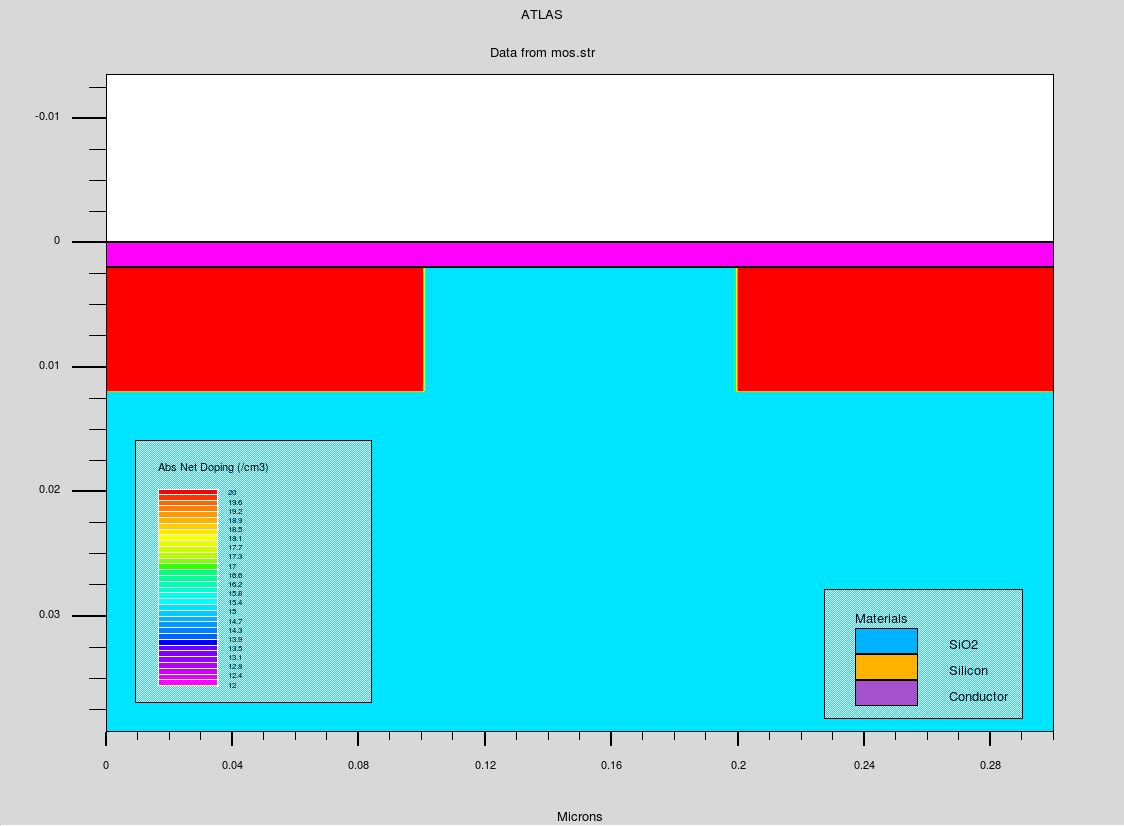
\includegraphics[width=300pt]{Images/Simu1-Dopage.png}
\caption{Image des différentes régions et dopages générés par le logiciel}
\label{transistortonyplot}
\end{figure}

Nous avons ainsi une modélisation 2D du transistor, comme le montre la Figure \ref{transistortonyplot}.

On précise ensuite au logiciel les différents contacts que nous allons utiliser, on obtient ainsi l'image en Figure \ref{TransistorFull}

\begin{figure}[H]
    \centering
    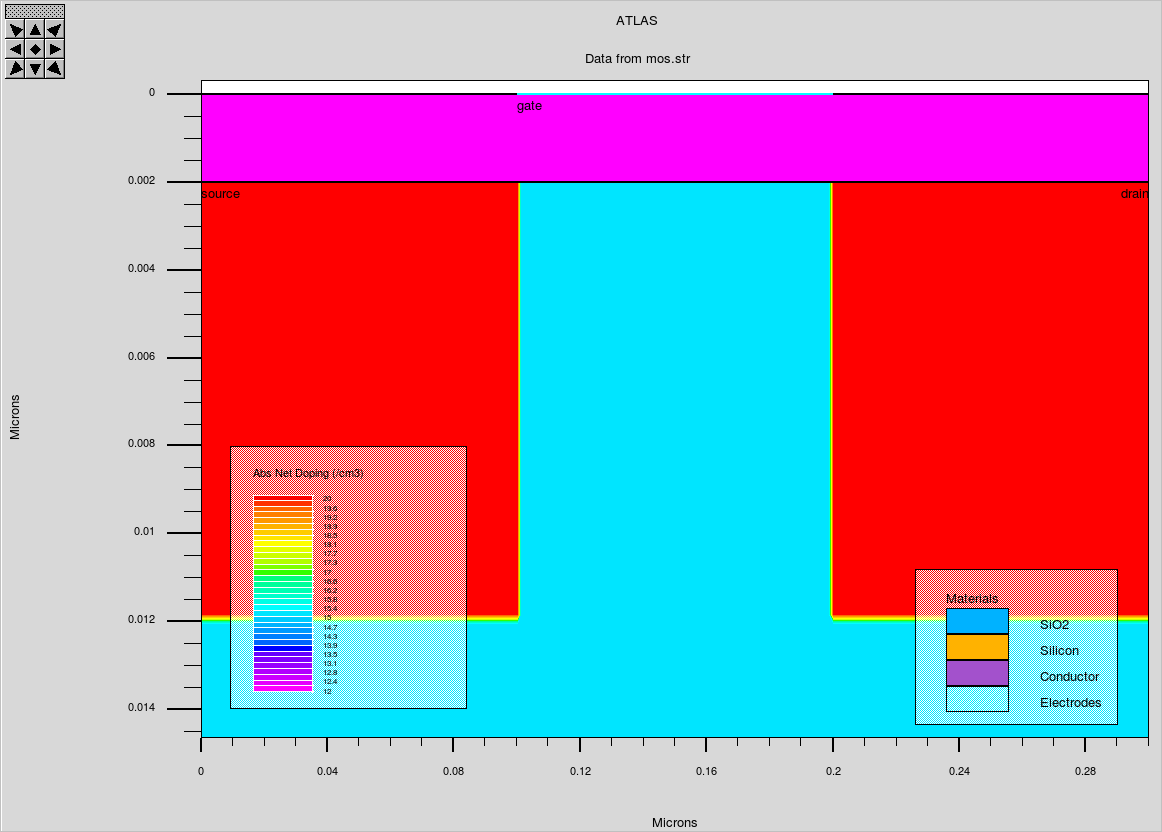
\includegraphics[width=300pt]{Images/TransistorFull.png}
    \caption{Image des régions, du dopage ainsi que des contacts générée par le logiciel}
    \label{TransistorFull}
\end{figure}

Maintenant que notre transistor est modélisé, nous allons pouvoir réaliser des simulations en jouant avec les différentes tensions appliquées.

\section{Tracés de caractéristiques}

En effet, il suffit ensuite d'ajouter quelques lignes au script afin de tracer des courbes, comme le montre la figure \ref{logIdVgmeshfin}.

\noindent\fbox{
\begin{minipage}{\textwidth}
    \noindent\texttt{output charge band.param ex.field ey.field jx.tot con.band val.band}
    \vspace{0.3cm}

    \noindent\texttt{solve init\\
    save outfile = nmos1.str}
    \vspace{0.3cm}

    \noindent\texttt{solve vgate = 0 vdrain = 0 vstep = 0.1 vfinal = 1 name = drain\\
    save outfile = nmos2.str}
    \vspace{0.3cm}

    \noindent\texttt{log outfile = idvg\_vds1.log\\
    save outfile = nmos3.str\\
    solve vgate = 0 vdrain = 1 vstep = 0.1 vfinal = 2 name = gate\\
    extract name="vt" (xintercept(maxslope(curve(abs(v."gate"),abs(i."drain")))) \ }

    \hspace{1cm} \texttt{- abs(ave(v."drain"))/2.0)}\\
    \texttt{extract name="subvt" \ }

    \hspace{1cm} \texttt{ 1.0/slope(maxslope(curve(abs(v."gate"),log10(abs(i."drain")))))}
\end{minipage}}

\begin{figure}[H]
\centering
    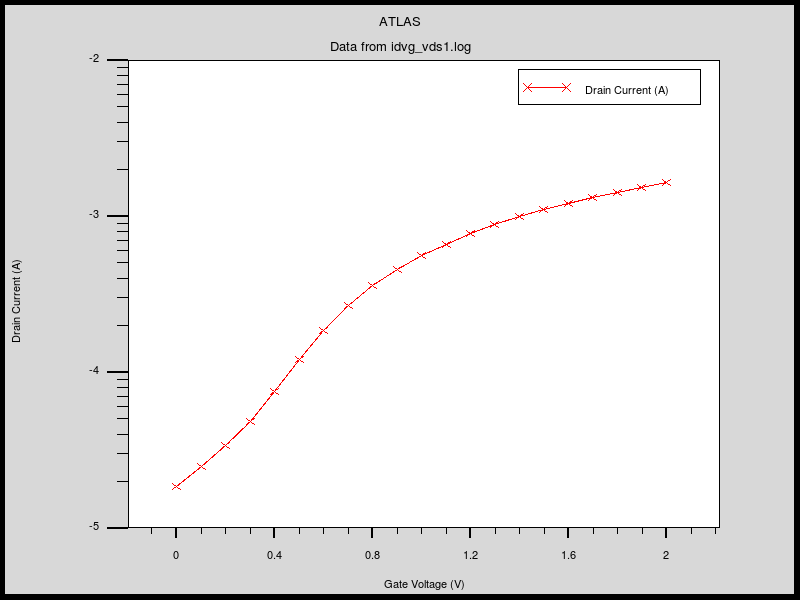
\includegraphics[width=300pt]{Images/MeshFin.png}
    \caption{Caractéristique logarithmique $\log(I_d(V_g))$}
    \label{logIdVgmeshfin}
\end{figure}

\section{Extraction des paramètres}
A partir de ce graphe il est possible d'extraire différents paramètres. Par exemple, pour $V_{ds}=50mV$, on trouve, pour la tension de seuil, la pente sous le seuil, le courant de saturation et le courant à vide :

\begin{tableau}[H]
\centering
\begin{tabular}{|c|c|}
\hline
$V_t$&$500mV$\\
\hline
$SubV_t$&$170mV/decade$\\
\hline
$I_{sat}$&$20mA$\\
\hline
$I_{off}$&$20\mu A$\\
\hline
\end{tabular}
\caption{Caractéristiques avec un maillage fin pour $V_{ds}=50mV$}

Ces valeurs sont cohérentes avec les ordres de grandeurs fournis dans le cours de composants.

\end{tableau}


\chapter{Optimisation du maillage}

Nous avons pu voir lors des calculs précédents qu'avec le maillage proposé initialement, l'obtention de points est très longue. En effet, le maillage est beaucoup trop fin, en particulier à des endroits où il n'a pas besoin de l'être. Par exemple le maillage n'a pas besoin d'être précis loin en profondeur, ni loin des interfaces. Par contre, proche des interfaces il faut qu'il soit fin pour bien représenter les changements brusques.
 
\section{Ecriture des modifications}
\vspace{0.3cm}

On modifie alors le maillage comme suit :
\vspace{0.3cm}

\noindent\fbox{
\begin{minipage}{\textwidth}
    \noindent\texttt{mesh space.mult = 1.0\\
    x.mesh loc = 0.0 spac = 0.005\\
    x.mesh loc = 0.1 spac = 0.001\\
    x.mesh loc = 0.2 spac = 0.001\\
    x.mesh loc = 0.3 spac = 0.005\\
    y.mesh loc = 0.000 spac = 0.0001\\
    y.mesh loc = 0.002 spac = 0.001\\
    y.mesh loc = 0.020 spac = 0.01\\
    y.mesh loc = 1.002 spac = 0.01}
\end{minipage}}
\vspace{0.3cm}

\section{Tracé de la caractéristique}

On peut ainsi également tracer la caractéristique obtenue avec ce maillage, en figure \ref{logIdVgmeshopti}

\begin{figure}[H]
    \centering
    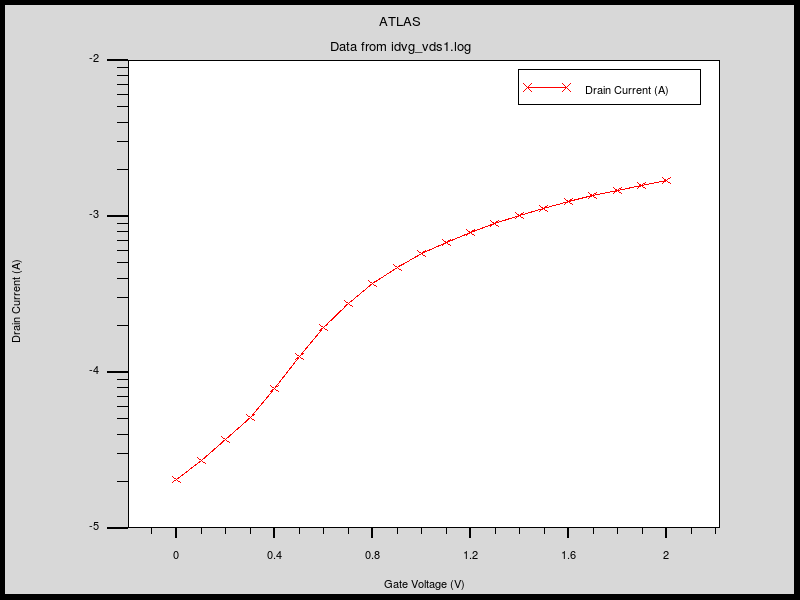
\includegraphics[width=300pt]{../meshOpti1/Log.png}
    \caption{Caractéristique $\log(I_g(V_g))$ obtenue avec un maillage optimisé.}
    \label{logIdVgmeshopti}
\end{figure}
 La courbe ressemble fortement à celle trouvée précédemment, avec le maillage fin, donc optimiser le maillage ne semble pas être destructeur.

\section{Extraction des paramètres}

On peut également extraire des paramètres de ce tracé, comme avec le maillage fin. On trouve ainsi :

\begin{tableau}[H]
\centering
\begin{tabular}{|c|c|}
\hline
$V_t$&$500mV$\\
\hline
$SubV_t$&$170mV/decade$\\
\hline
$I_{sat}$&$2mA$\\
\hline
$I_{off}$&$22\mu A$\\
\hline
\end{tabular}
\caption{Caractéristiques avec un maillage optimisé avec $V_{ds}=50mV$}
\end{tableau}

\section{Comparaison des deux maillages}

Les valeurs trouvées sont cohérentes avec les valeurs précédentes, ce qui laisse à penser que le maillage optimisé ne réduit pas la précision.

Il convient ensuite de comparer les deux courbes obtenues, pour vérifier si le maillage moins précis donne le même résultat que le maillage fin. Cette comparaison est fournie en Figure \ref{compMesh}.

\begin{figure}[H]
  \centering
  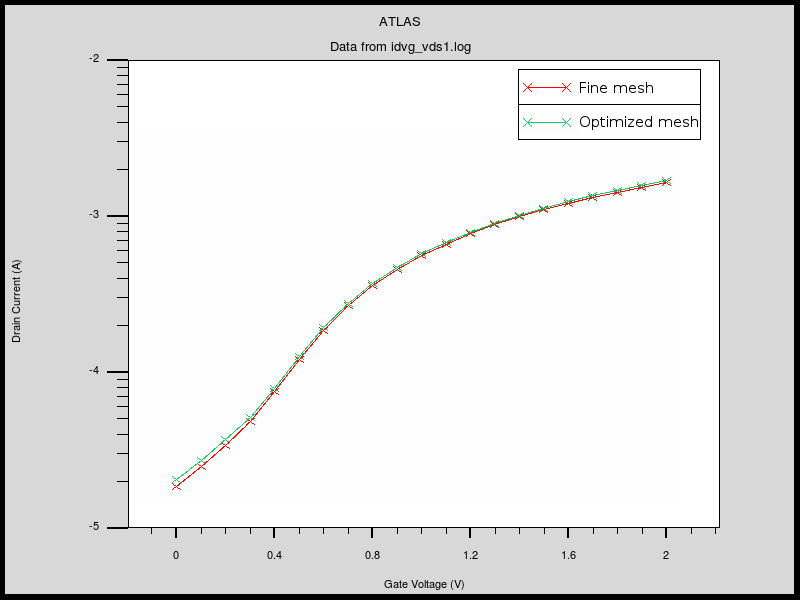
\includegraphics[width=250pt]{Images/MeshFinEtOpti.png}
  \caption{Comparaison des deux maillages pour $V_{ds}=50mV$}
  \label{compMesh}
\end{figure}


Sur ce graphe, on remarque que malgré les légères différences, les courbes sont très semblables et cela semble rentable d'un point de vue gain de temps de simulation par rapport aux possibles faibles erreurs engendrées. Le maillage optimisé est adapté pour réaliser plusieurs simulations rapides, lors de phases de tests. Puis, il est possible d'utiliser un maillage plus précis par la suite, lorsque l'on souhaite plus de précisions sur les mesures, lorsque les paramètres avec le maillage optimisé donnent des résultats proche de ce que l'on souhaite.

% \section{Extraction des paramètres}
% A partir des caractéristiques tracées, nous pouvons remonter à certains paramètres. Par exemple, SS et DIBL.
%


\chapter{Une autre architecture : FDSOI}

\section{Position du problème}

On passe à une architecture Fully Depleted Silicon On Insulator (FDSOI), qui permet de limiter la variation de $V_t$ avec la réduction de la longueur de grille, qui apparaît avec l'architecture Bulk.  Le schéma représentant cette architecture est donné en Figure \ref{SchemaFDSOI}.

\begin{figure}[H]
    \centering
    \begin{tikzpicture}
        \fill [color=gray!20] (3,5)--(7,5)--(7,4.8)--(3,4.8)--cycle;
        \fill [color=black] (3,5)--(7,5)--(7,5.2)--(3,5.2)--cycle;
        \draw [thick] (0,5)--(10,5);
        \draw (3,5)--(3,3)--(0,3);
        \draw (1.5,4)node{n};
        \draw (7,5)--(7,3)--(10,3);
        \draw (8.5,4)node{n};
        \draw (5,4.8)node[below]{Canal};
        \draw (3,5)--(3,6)--(7,6)--(7,5)--cycle;
        \fill [color=gray!30] (0,1)--(0,2)--(10,2)--(10,1)--cycle;
    \end{tikzpicture}
    \caption{Schéma d'un transistor FDSOI}
    \label{SchemaFDSOI}
\end{figure}

Nous avons modélisé ce transistor sur Silvaco.

\section{Tracé des caractéristiques}

On peut ainsi tracer les caractéristiques :

\begin{figure}[H]
    \centering
    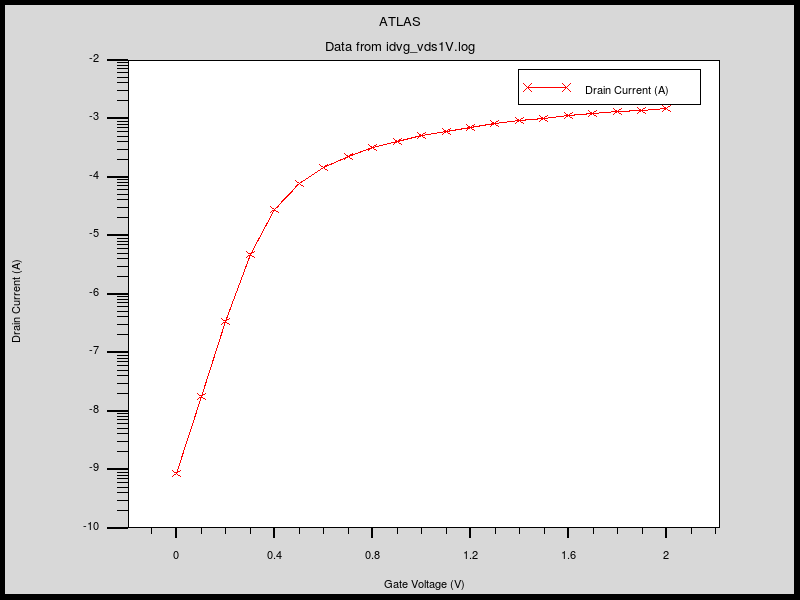
\includegraphics[width=300pt]{../FDSOI/LogIdVg.png}
    \caption{Caractéristiques $\log(I_d(V_g))$ pour $V_d$ faible (en rouge) et $V_d$ fort (en vert)}    
\end{figure}

En comparant la courbe à celle trouvée pour l'architecture bulk, on remarque qu'elle est plus lisse, on discerne bien deux parties presque linéaires, alors que c'était moins le cas pour l'architecture bulk.

\section{Extraction des paramètres}

On peut, à partir de cette courbe déduire : 

\begin{tableau}[H]
\centering
\begin{tabular}{|c|c|}
\hline
$V_t$&$350mV$\\
\hline
$SubV_t$&$170mV/decade$\\
\hline
$I_{sat}$&$1mA$\\
\hline
$I_{off}$&$1 nA$\\
\hline
\end{tabular}
\caption{Caractéristiques du FDSOI avec $V_{ds}=1V$}
\end{tableau}

On remarque, en comparant aux valeurs pour le transistor bulk que si la tension de seuil et la pente sous le seuil sont relativement proche, les courants sont différents. En particulier le courant $I_{off}$ qui est très faible, ce qui est un bon point point pour la consommation d'energie lorsque le transistor n'est pas actif. De plus, le courant de saturation est également plus faible, donc même en utilisation le transistor consommera moins d'énergie.

\chapter{Etude plus approfondie}

\section{Comparaison NMOS et PMOS}

Jusqu'à présent toutes nos études ont été réalisées sur des transistors NMOS, cependant, il est possible de voir la différence entre NMOS et PMOS en changeant les zones de dopage. 

Les tracés des caractéristiques $Id(V_g)$ donnent : 

\begin{figure}[H]
\centering
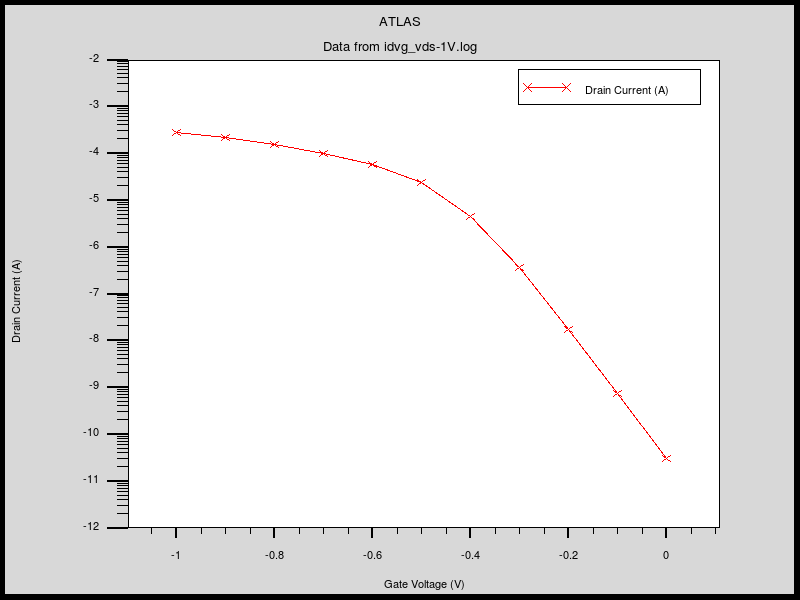
\includegraphics[width=170pt]{../15Decembre/pmosIDs_Vg.png}
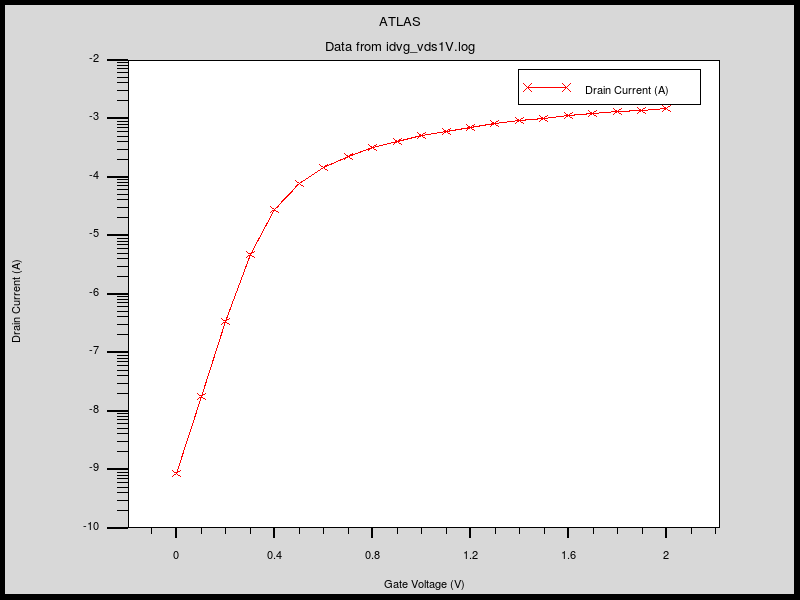
\includegraphics[width=170pt]{../15Decembre/Ids_Vg.png}
\caption{Comparaison des caractéristiques de PMOS et NMOS}
\end{figure}

La caractéristique pour PMOS est le symétrique de celle du NMOS, les valeurs de $V_t$ sont similaires en valeur absolu et opposées (négative pour le PMOS).

\section{Bandes de conduction}

Grâce à TonyPlot, nous avons pu tracer les bandes de conduction dans une coupe le long du canal.

Tout d'abord, pour $V_d=50mV$ :
\begin{figure}[H]
\centering
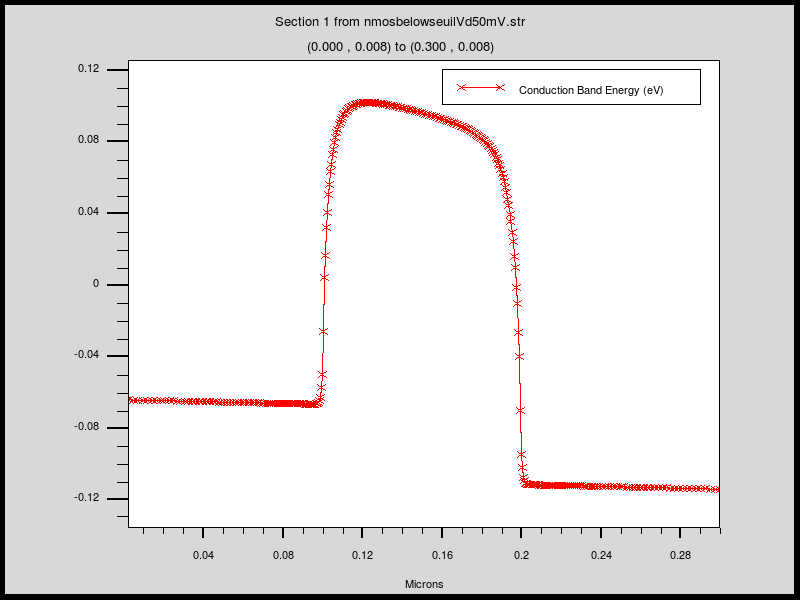
\includegraphics[width=170pt]{../15Decembre/NMOS/nmosbelowseuilVd50mV_Condband.png} 
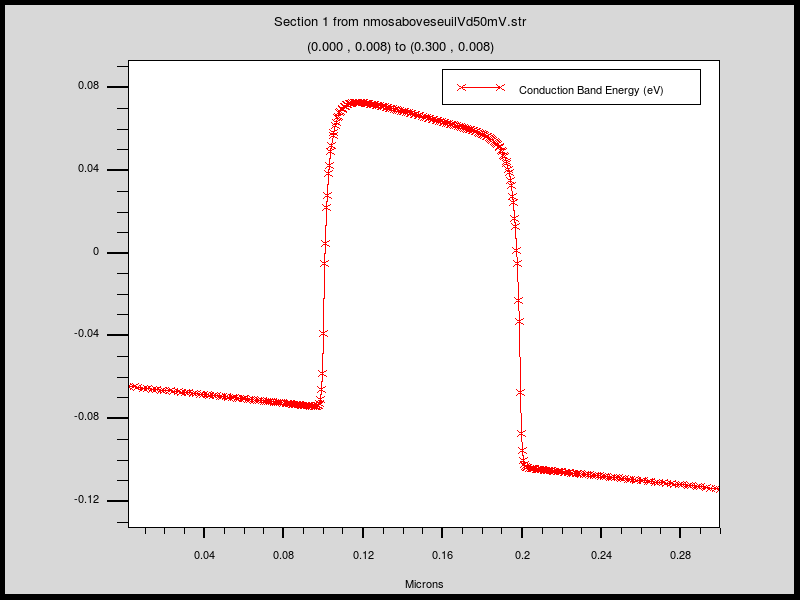
\includegraphics[width=170pt]{../15Decembre/NMOS/nmosaboveseuilVd50mV_condband.png}
\caption{Champ Electrique pour $V_d=50mV$ sous le seuil puis au-dessus du seuil}
\end{figure}

Puis pour $V_d=1V$ :

\begin{figure}[H]
\centering
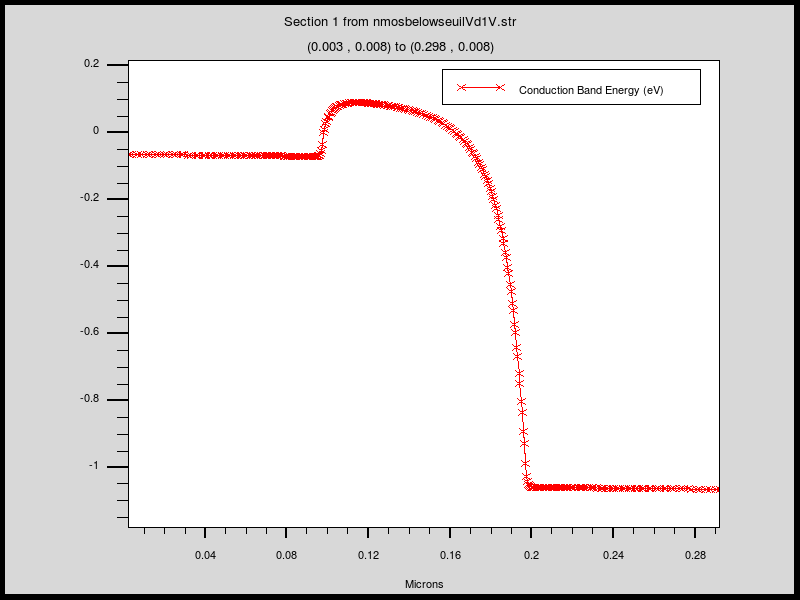
\includegraphics[width=170pt]{../15Decembre/NMOS/nmosbelowseuilVd1V_condband.png} 
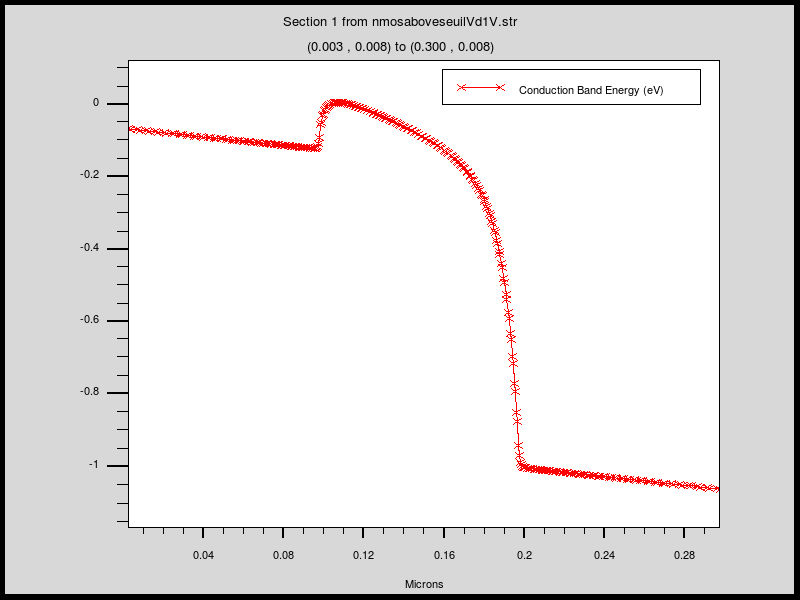
\includegraphics[width=170pt]{../15Decembre/NMOS/nmosaboveseuilVd1V_condband.png}
\caption{Champ Electrique pour $V_d=1V$ sous le seuil puis au-dessus du seuil}
\end{figure}

La bande de conduction reflètent le comportement physique du transistor par application d'un potentiel. Pour $V_d$ faible, les courbes correspondent à ce que la théorie prédit pour une jonction npn, avec le décalage induit par la présence de $V_g$ pour $V_g>V_t$. Pour $V_d$ fort, la courbe est très déformée du à la grande différence de potentiel, il n'y a plus vraiment de partie plate dans la partie p. Cel devrait avoir un influence certaine sur le champ à l'intérieur du tranistor.

\section{Champ électrique}

Nous pouvons effectivement représenter le champ électrique :

Tout d'abord, pour $V_d=50mV$ :
\begin{figure}[H]
\centering
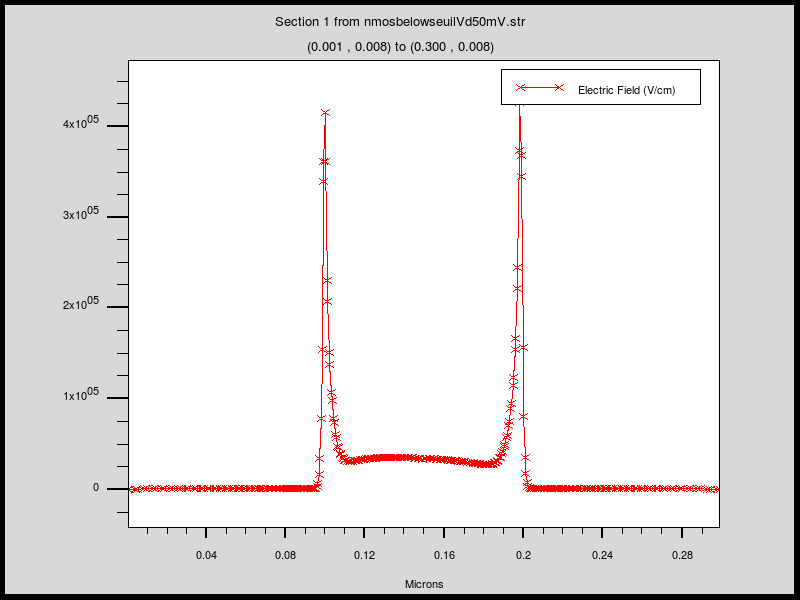
\includegraphics[width=170pt]{../15Decembre/NMOS/nmosbelowseuilVd50mV_Efield.png} 
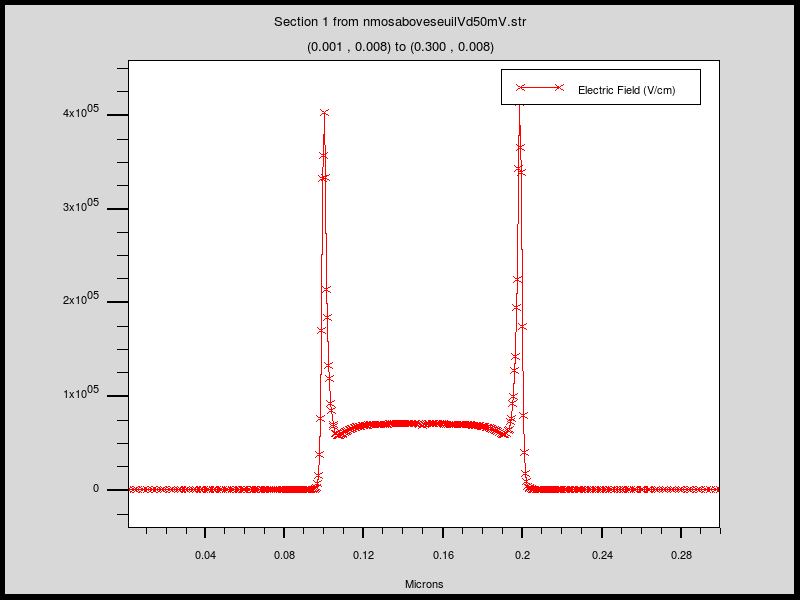
\includegraphics[width=170pt]{../15Decembre/NMOS/nmosaboveseuilVd50mV_Efield.png}
\caption{Champ Electrique pour $V_d=50mV$ sous le seuil puis au-dessus du seuil}
\end{figure}

Puis pour $V_d=1V$ :

\begin{figure}[H]
\centering
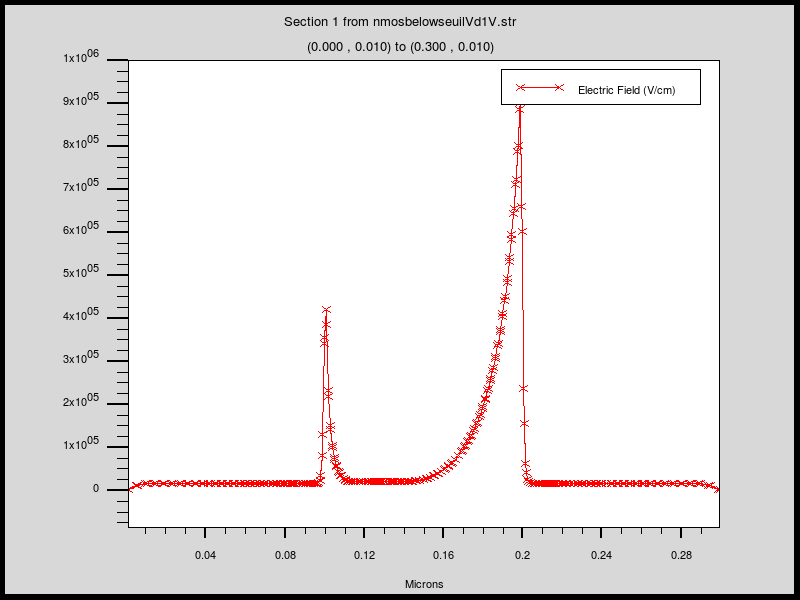
\includegraphics[width=170pt]{../15Decembre/NMOS/nmosbelowseuilVd1V_Efield.png} 
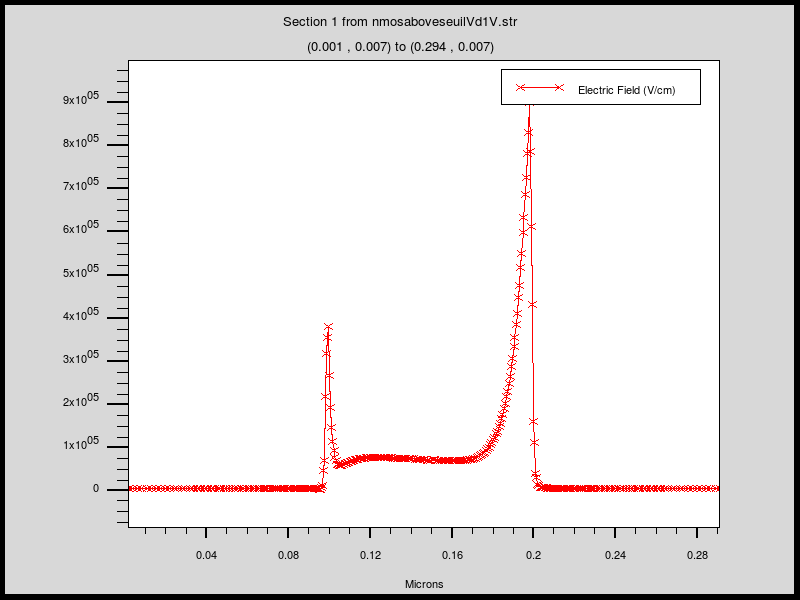
\includegraphics[width=170pt]{../15Decembre/NMOS/nmosaboveseuilVd1V_Efield.png}
\caption{Champ Electrique pour $V_d=1V$ sous le seuil puis au-dessus du seuil}
\end{figure}

On remarque qu'appliquer un $V_d$ fort renforce l'amplitude du pic correspondant au drain. En effet, le champ electrique et le potentiel sont liés par la relation :

\[\vec{E}=-grad(V)\]

Ce qui implique qu'augmenter la différence de potentiel entre le drain et le silicium dopé augmente le champ electrique. Les résultats sont donc conforme à ce que prédit la théorie. De plus, on remarque qu'au-dessus du seuil, le champ electrique ne retombe pas à 0 entre les deux pics, ce qui implique un déplacement des porteurs, et donc l'établissement d'un courant pour $V_g>V_t$.
\vspace{0.5cm}

\section{Concentration des porteurs}

Justement, nous pouvons également tracer la concentration des porteurs dans le transistor :

Tout d'abord, pour $V_d=50mV$ :
\begin{figure}[H]
\centering
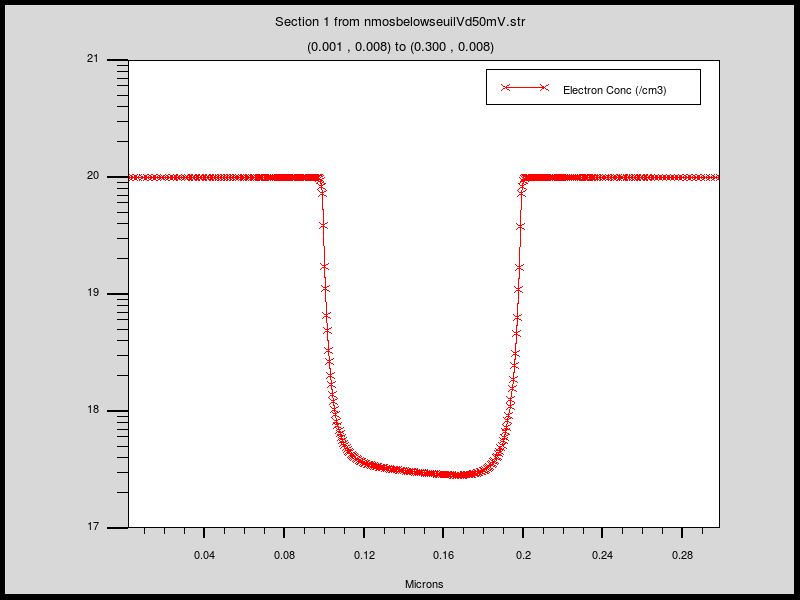
\includegraphics[width=170pt]{../15Decembre/NMOS/nmosbelowseuilVd50mV_econc.png} 
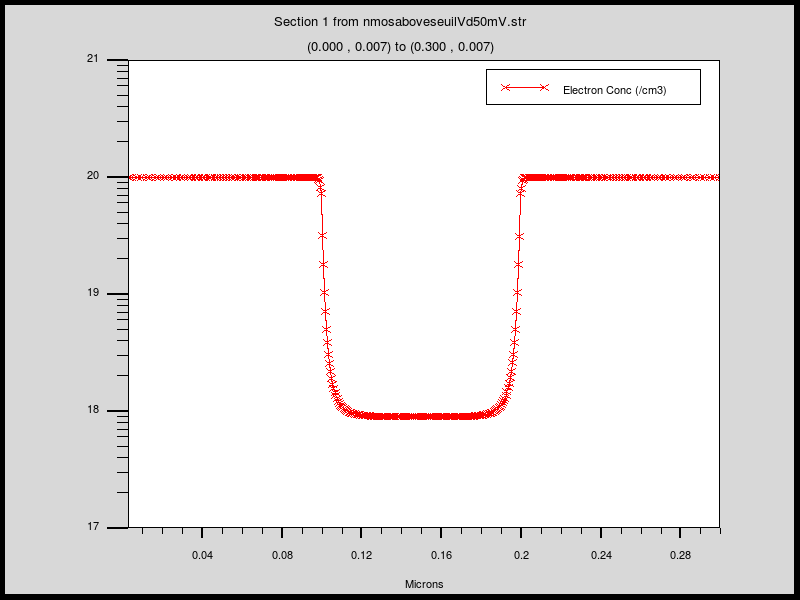
\includegraphics[width=170pt]{../15Decembre/NMOS/nmosaboveseuilVd50mV_econc.png}
\caption{Champ Electrique pour $V_d=50mV$ sous le seuil puis au-dessus du seuil}
\end{figure}

Puis pour $V_d=1V$ :

\begin{figure}[H]
\centering
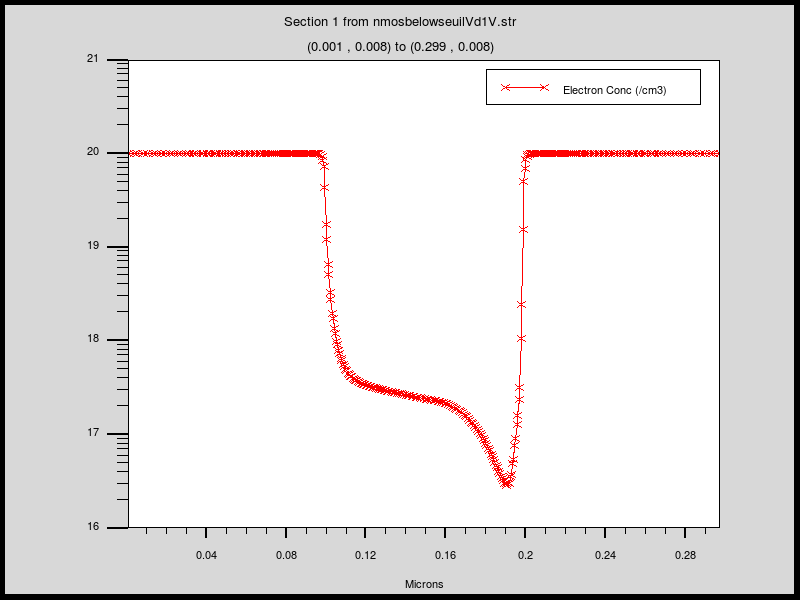
\includegraphics[width=170pt]{../15Decembre/NMOS/nmosbelowseuilVd1V_econc.png} 
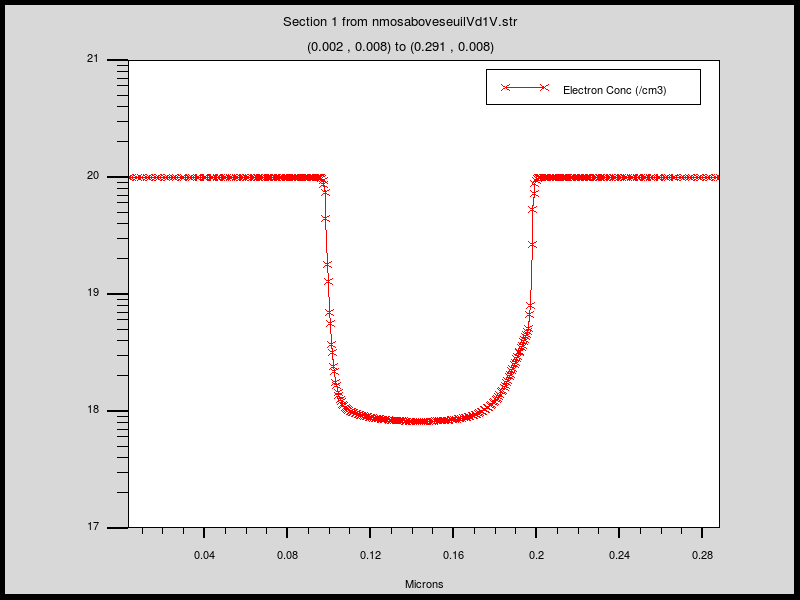
\includegraphics[width=170pt]{../15Decembre/NMOS/nmosaboveseuilVd1V_econc.png}
\caption{Champ Electrique pour $V_d=1V$ sous le seuil puis au-dessus du seuil}
\end{figure}

On multiplie la concentration des porteurs environ par deux en dépassant le seuil, dans les deux cas. Cependant, on remarque une différence pour $V_d$ fort. Un creux présent sous le seuil qui disparait lors au passage du seuil. Sous le seuil, les porteurs ne peuvent pas passer et sont naturellement repoussés par le drain. Au-dessus du seuil, en revanche, les porteurs sont attirés par le drain du fait du champ qui règne au sein du canal, ce qui induit le courant car :

\[\rho=\varepsilon_0div(\vec{E})\]


\chapter*{Conclusion}
\addcontentsline{toc}{chapter}{Conclusion}

La simulation est une grande part de la conception dans le sens où entrer quelques lignes  de code dans un programme est bien moins lourd que de mettre en place des protocoles expérimentaux de fabrication et de mesures pour des technologies novatrices dont les caractéristiques sont encore très peu connues. Cependant cela requiert des outils de simulation relativement puissant afin de modéliser tous les effets, mais aussi de solides bases théoriques qui indiquent les équations qui décrivent le comportement des dispositifs et composants. Nous avons pu observer cela via l'étude de composants relativement simples, mais dont l'étude complète et poussée est bien plus rapide via simulation que via les calculs vu en cours, ou même que via des outils de caractérisation de transistors déjà fabriqués.

\end{document}
